\section{Descrizione del progetto}
Il progetto scritto in Scala prevede di andare ad affiancare, alla macchinetta del caffè gestita in ASMETA, un distributore automatico di bevande energetiche.
In particolar modo si è progettato un sistema con queste specifiche:
\begin{itemize}
	\item Ogni distributore automatico può essere impostato per funzionare in una lingua piuttosto che in un'altro: nel codice è gestitata solamente la possibilità di introdurre distirbutori automatici in lingua italiana e in lingua inglese.
	
	\item Questi distributori possono gestire le seguenti bevande energetiche (\textit{energy drink}):
	\begin{itemize}
		\item RedBull
		\item Monster
		\item Gatorade
		\item Italian
	\end{itemize}
	Ognuno di questi prodotti sarà caratterizzato dai seguenti campi descrittivi:
	\begin{itemize}
		\item prezzo
		\item volume (espresso in cl)
		\item data di scadenza
		\item insieme di tags, che permettono di esprimere le caratteristiche salienti di ognuno degli energy drink
	\end{itemize}
\end{itemize}

Ogni distributore andrà ad offrire le seguenti funzionalità:
\begin{itemize}
	\item Acquisto dei prodotti disponibili, regalando i prodotti scaduti: in particolare la macchinetta sarà in grado di fornire resto esatto al cliento (oppure tutta la somma di denaro inserita nel caso di prodotto scaduto).
	\item Mostrare l'elenco dei prodotti disponibili all'interno del distirbutore (identificato tramite ID), unitamente al numero di pezzi disponibili, come si vede in figura ~\ref{fig:AvailableProducts}.
	\begin{figure}[h]
		\centering
		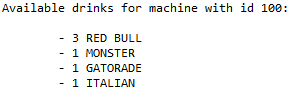
\includegraphics[width=0.3\textwidth]{Immagini/ShowVendingMachine.png}
		\caption{Prodotti disponibili}
		\label{fig:AvailableProducts}
	\end{figure}
	\item Possibilità di cercare un prodotto tramite tag, per poter così trovare l'energy drink più adatto ad ogni evenienza
	\item Aggiunta di energy drink all'interno del distributore: nello specifico, l'aggiunta di un nuovo prodotto, avviene all'interno di una struttra definita come un array di Queue (ovvero una matrice), che non fa altro che andare a riprodurre la fisionomia di un distirbutore reale.
\end{itemize}

\section{Gerarchia delle classi}
Nella applicazione realizzata sono stati realizzata due gerarchie facendo uso dei \textit{trait}: i trait in Scala corrispondono alle interfaccie in Java, ovvero permettono di definire la firma di ogni classe che ne implementa la struttura.
Nel nostro caso abbiamo due strutture gerarchiche, gestite tramite traits, mostrate con un grafo ad "albero" nell'immagine seguente (figura ~\ref{fig:classi&traits}).

\begin{figure}[h]
	\centering
	\subfloat[][\emph{Energy drink}]
	{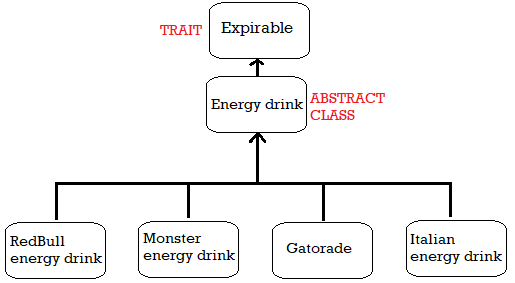
\includegraphics[width=.45\textwidth]{Immagini/EnergyDrink.png}} \quad
	\subfloat[][\emph{Expirable trait}]
	{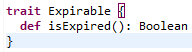
\includegraphics[width=.45\textwidth]{Immagini/ExpirableTrait.png}} \\
	\subfloat[][\emph{Vending machine}]
	{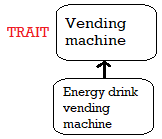
\includegraphics[width=.3\textwidth]{Immagini/VendingMachine.png}} \quad
	\subfloat[][\emph{Vending machine trait}]
	{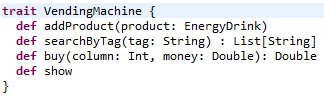
\includegraphics[width=.45\textwidth]{Immagini/VendingMachineTrait.png}}
	\caption{Classi e trait}
	\label{fig:classi&traits}
\end{figure}


\newpage
\section{Filter}
Per quanto riguarda la funzionalità di ricerca delle bevande in base ai tag, è stato utile la funzionalità \textit{filter}.

Il comando di filter è utile nel momento in cui si vogliono filtrare gli elemnti di una certa collezione (lista, array, vettore etc), andando a creare una nuova collezione contenente solamente gli elementi che rispettano il criterio di filtraggio definito in maniera custom.

Nella nostra applicazione siamo andati a filtrare l'elenco dei tag di ogni prodotto: il filtraggio è stato pensato per mantenere solamente i tag contenenti al loro interno il tag cercato dall'utente tramite tastierino di input.

\begin{figure}[h]
	\centering
	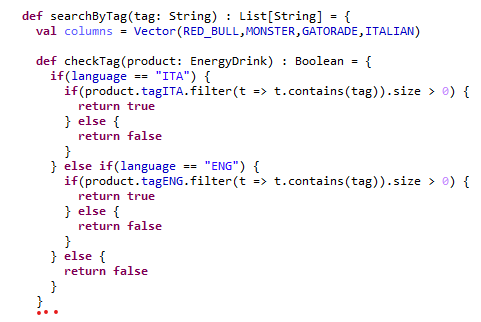
\includegraphics[width=0.5\textwidth]{Immagini/Filter.png}
	\caption{Utilizzo comando \textit{filter} nella nostra applicazione}
	\label{fig:filter}
\end{figure}
Come si vede in figura ~\ref{fig:filter}, in base alla tipologia di lingua con cui il distributore è stato impostato, si va a cercare nei rispettivi tag, solamente quelli che contengono la parola chiave cercata: in particolare, se il risultato dell'operazione di filter è un vettore con una lunghezza maggiore di 0, significa che il prodotto in esame soddisfa il tag cercato, e quindi può essere mostrato all'utente. Questa operazione di filtraggio viene poi ripetuta per ogni tipologia di prodotto disponibile, ovvero per ogni colonna. 

Una volta effettuato il filtraggio siamo andati a considerare solamente i prodotti il cui risultato dall'operazione di filter non fosse un vettore nullo: questo corrisponde infati al considerare solamente i prodotti che contengono il tag cercato, notificando poi all'utente la loro tipologia, tramite una stampa a display.
\section{Match - sealed}
\subsection{Match}
Il \textit{pattern matchin} rappresenta una struttura per verificare il valore aassunto da una variabile, tramite un pattern: si tratta in sostanza di una versione leggermente più potente del construtto \textit{switch} di Java.
Nella nostra applicazione si è pensato di andare ad utilizzare il \textit{pattern matching} in due situazioni:
\begin{itemize}
	\item \textit{Pattern guard}: nell'andare a definire se un prodotto è considerabile come normo, ipo o iper calorico, si è fatto uso di un pattern guard, sfruttando anche la potenzialità aggiuntiva di poter aggiungere una condizione dopo il pattern, tramite la dicitura \textit{if<boolean expression>}, che permette di rendere più specifico ogni singolo case.
	\item \textit{Matching on classes}: per la funzionalità di aggiunta di nuovi prodotti all'interno del distributore automatico, si era pensato di utilizzare un \textit{pattern match} per poter distinguere la tipologia specifica del prodotto aggiunto. Alla fine la scelta è però ricaduta sull'utilizzo del comando \textit{isInstanceOf}.
\end{itemize}
\subsection{Sealed}
Classi e traits possono essere segnati come \textit{sealed}: questo significa che tutti i sotto tipi devono essere dichiarati all'interno dello stesso file, garantendo che tutti i sottotipi siano conosciuti e noti.
\begin{figure}[h]
	\centering
	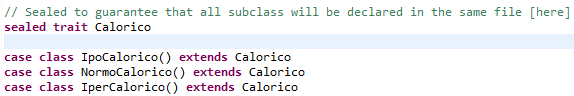
\includegraphics[width=0.5\textwidth]{Immagini/Sealed.png}
	\caption{Sealed}
	\label{fig:sealed}
\end{figure}
